%
% $RCSfile: mind_and_brain.tex,v $
%
% Copyright (C) 2002-2008. Christian Heller.
%
% Permission is granted to copy, distribute and/or modify this document
% under the terms of the GNU Free Documentation License, Version 1.1 or
% any later version published by the Free Software Foundation; with no
% Invariant Sections, with no Front-Cover Texts and with no Back-Cover
% Texts. A copy of the license is included in the section entitled
% "GNU Free Documentation License".
%
% http://www.cybop.net
% - Cybernetics Oriented Programming -
%
% http://www.resmedicinae.org
% - Information in Medicine -
%
% Version: $Revision: 1.1 $ $Date: 2008-08-19 20:41:07 $ $Author: christian $
% Authors: Christian Heller <christian.heller@tuxtax.de>
%

\paragraph{Mind and Brain}
\label{mind_and_brain_heading}
\index{Mind and Brain}
\index{Knowledge and System Control}
\index{Software as Passive Knowledge and Active Control}

A first observation, when looking at human beings from a philosophical
perspective, is the separation of \emph{Mind} and \emph{Brain} (Body) (figure
\ref{staticsdynamics_figure}). Accordingly, CYBOP treats computers as
\emph{Systems} owning and processing \emph{Knowledge}. This is not unlike the
idea of \emph{Agent} systems owning a \emph{Knowledge Base} (section
\ref{agent_oriented_programming_heading}). All abstract knowledge that humans
make up belongs to their mind. The brain is merely a physical carrier of
knowledge.

\begin{figure}[ht]
    \begin{center}
        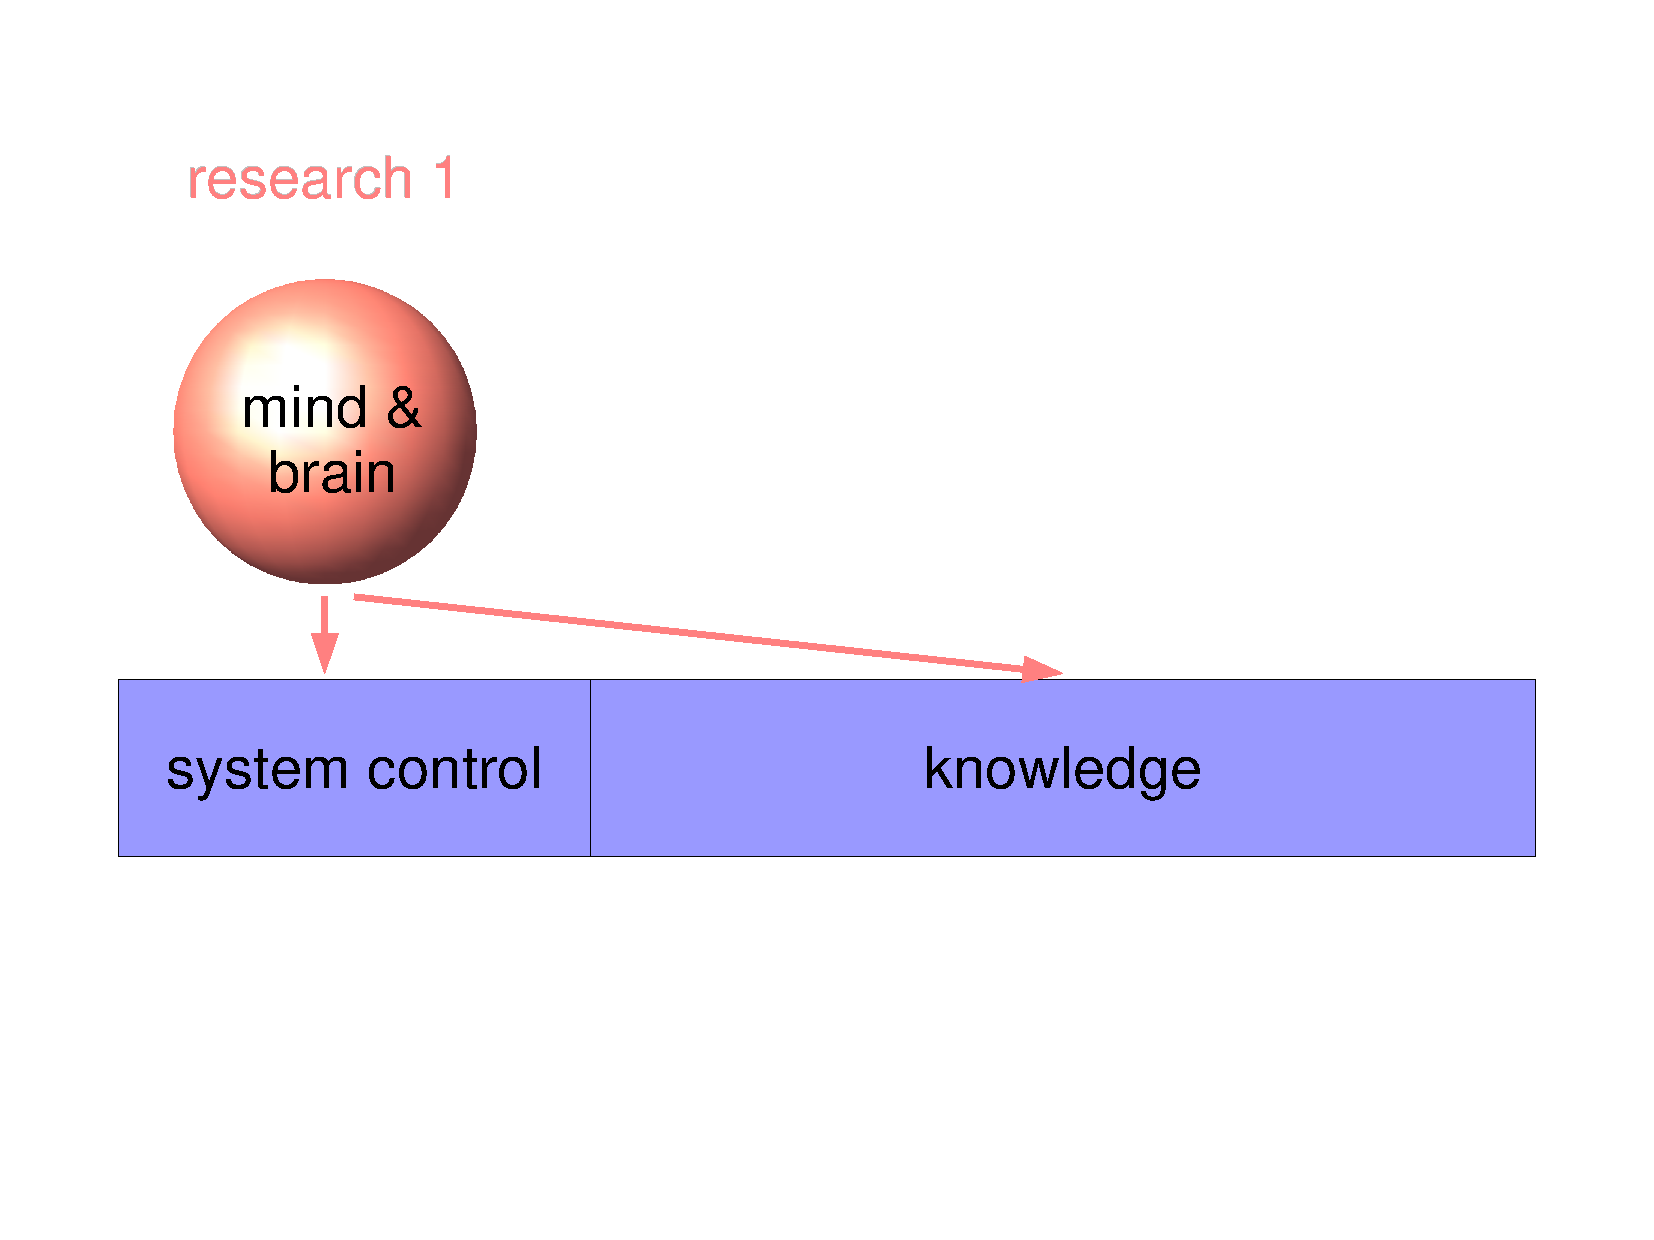
\includegraphics[scale=0.3,angle=-90]{graphic/staticsdynamics.pdf}
        \caption{Separation of Mind/ Brain Leading to Knowledge/ System Control}
        \label{staticsdynamics_figure}
    \end{center}
\end{figure}

Another conclusion resulting from this first observation is that there should
actually be two kinds of software: one representing \emph{passive} knowledge
and the other \emph{actively} controlling a system, close to hardware.

Chapter \ref{statics_and_dynamics_heading} deals with this topic.
